\section{Introduction}\label{sec:intro}
Transformer~\cite{vaswani2017attention} has been dominant in deep learning research for recent years. 
It works as a backbone module in many fundamental models, achieving outstanding performance in various application scenarios. 
Currently, the most successful language models like BERT~\cite{devlin2019bert} and GPT~\cite{brown2020language} are built based on the Transformer or its variants~\cite{child2019generating,dai2019transformer}, which outperforms classic recurrent neural network (RNN) architectures on both effectiveness and efficiency. 
In the field of computer vision, the Vision Transformers (ViTs)~\cite{dosovitskiy2021an,liu2021swin,arnab2021vivit} have achieved better performance in many image recognition and understanding tasks compared to convolutional neural networks (CNNs).
Recently, the Transformer-based models have been designed for the structured data in different applications, including the Informer~\cite{zhang2021informer} for time series broadcasting, the Graphormer~\cite{ying2021transformers} for molecular representation, the Set-Transformer~\cite{lee2019set} and Point-Transformer~\cite{zhao2021point} for point cloud modeling, and so on.
More and more cases show the tendency that the Transformer is becoming a natural and indispensable choice when developing deep learning models.

\begin{table}[t]
    \caption{A comparison for transformers and our sliceformer on their ``attention'' mechanisms. For simplification, we just show one attention head for each model, in which the input $\bm{X}\in\mathbb{R}^{N\times d}$, the value matrix $\bm{V}=\bm{X}\bm{W}_V\in\mathbb{R}^{N\times D}$, the query matrix $\bm{Q}=\bm{X}\bm{W}_Q\in\mathbb{R}^{N\times D}$, and the key matrix $\bm{K}=\bm{X}\bm{W}_K\in\mathbb{R}^{N\times D}$.}
    \label{tab:cmp}
    \centering
    \small{
    \begin{threeparttable}
    {\def\arraystretch{1.7}\tabcolsep=6pt
    \begin{tabular}{l|lll}
    \hline\hline
    Model & 
    $\text{Attention}(\bm{V};\bm{Q},\bm{K})$ & 
    Complexity & 
    Attention Structure \\
    \hline
    Transformer~\cite{vaswani2017attention}  & 
    $\text{Softmax}\left(\frac{\bm{Q}\bm{K}^{\top}}{\sqrt{D}}\right)\bm{V}$ & 
    $\mathcal{O}(DN^2)$ & 
    Dense + Row-stochastic\\
    SparseTrans~\cite{child2019generating} & 
    $\text{Local2D-Softmax}\left(\frac{\bm{Q}\bm{K}^{\top}}{\sqrt{D}}\right)\bm{V}$ & 
    $\mathcal{O}(DN^{1.5})$ &
    Sparse + Row-stochastic\\
    Longformer~\cite{beltagy2020longformer}   & 
    $\text{Local1D-Softmax}\left(\frac{\bm{Q}\bm{K}^{\top}}{\sqrt{D}}\right)\bm{V}$ &  
    $\mathcal{O}(DNL)$ &
    Sparse + Row-stochastic\\
    Reformer~\cite{kitaev2020reformer}     & 
    $\text{LSH-Softmax}\left(\frac{\bm{Q}\bm{K}^{\top}}{\sqrt{D}}\right)\bm{V}$ &  
    $\mathcal{O}(DN\log N)$ &
    Sparse + Row-stochastic\\
    CosFormer~\cite{zhen2022cosformer}    & 
    $(\bm{Q}_{\cos}\bm{K}_{\cos}^{\top}+\bm{Q}_{\sin}\bm{K}_{\sin}^{\top})\bm{V}$ & 
    $\mathcal{O}(\min\{DE_{QK},NE_{Q}\})$&
    Sparse\\
    Performer~\cite{choromanski2021rethinking}  & 
    $\phi_r(\bm{Q})\phi_r(\bm{K})^{\top}\bm{V}$ & 
    $\mathcal{O}(DNr)$ &
    Low-rank\\
    Linformer~\cite{wang2020linformer}    & 
    $\text{Softmax}\left(\frac{\bm{Q}\psi_r(\bm{K})^{\top}}{\sqrt{D}}\right)\psi_r(\bm{V})$ & 
    $\mathcal{O}(DNr)$ &
    Low-rank + Row-stochastic\\
    Sinkformer~\cite{sander2022sinkformers}   & 
    $\text{Sinkhorn}_{K}\left(\frac{\bm{Q}\bm{K}^{\top}}{\sqrt{D}}\right)\bm{V}$ & 
    $\mathcal{O}(KDN^2)$ &
    Dense + Doubly stochastic\\
    \hline
    \textbf{Sliceformer}  & 
    $\text{Sort}_{\text{col}}(\bm{V})$ & 
    $\mathcal{O}(DN\log N)$ &
    Sparse + Doubly stochastic\\
    \hline\hline
    \end{tabular}
    }
    \begin{tablenotes}
    \item[1] \footnotesize{``Local1D'' means considering the local data for a 1D sequence, while ``Local2D'' means considering the row-wise and column-wise local data for a sequence zigzagging in the 2D space. ``LSH'' denotes Locality-sensitive Hashing.}
    \item[2] \footnotesize{$\phi_r: \mathbb{R}^{D}\mapsto\mathbf{R}^r$, and $\phi_r(\bm{Q}),\phi_r(\bm{K})\in\mathbb{R}^{N\times r}$; $\psi_r: \mathbb{R}^{N}\mapsto\mathbf{R}^r$, and $\psi_r(\bm{K}),\psi_r(\bm{V})\in\mathbb{R}^{r\times D}$.}
    \item[3] $\bm{K}_{\cos}=\text{diag}(\{\cos\frac{\pi i}{2M}\}_{i=1}^{N})\text{ReLU}(\bm{K})$, $\bm{K}_{\sin}=\text{diag}(\{\sin\frac{\pi i}{2M}\}_{i=1}^{N})\text{ReLU}(\bm{K})$. So are $\bm{Q}_{\cos}$ and $\bm{Q}_{\sin}$. 
    $E_{QK}$ represents the number of nonzero elements in $\bm{Q}_{\cos}\bm{K}_{\cos}^{\top}$, while $E_Q$ represents the number of nonzero elements in $\bm{Q}_{\cos}$.
    \item[4] ``$\text{Sinkhorn}_{K}$'' means applying $K$-step Sinkhorn iterations.
    \item[5] Note that, our Sliceformer does not need the ``multi-head'' architecture because of the simplicity of sorting.
    \end{tablenotes}
    \end{threeparttable}
}
\end{table}

The popularity of the Transformer reflects the ``hegemony'' of the multi-head attention (MHA) mechanism~\cite{vaswani2017attention} behind it, which might be questionable in our opinion.
In particular, without strict theoretical support, the effectiveness of the Transformer is often attributed to the MHA mechanism.
This empirical but dominant opinion impacts the design and modification of the Transformer significantly.
As shown in Table~\ref{tab:cmp}, many efforts are made to $i)$ improve the efficiency of MHA, e.g., designing sparse or low-rank attention maps~\cite{child2019generating,kitaev2020reformer,wang2020linformer}, and $ii)$ enhance the interpretability of MHA, e.g., providing new understandings through the lens of kernel theory~\cite{tsai2019transformer,zhen2022cosformer} and optimal transport~\cite{tay2020sparse,sander2022sinkformers}.
Although some variants of Transformer challenge the sufficiency of MHA~\cite{dong2021attention,gu2021efficiently,ma2022mega}, they still take the MHA as a necessary module in their architectures. 
On the contrary, little attention is paid to studying the rationality and necessity of the MHA itself or, more ambitiously, replacing the MHA with a new surrogate. 
Recently, some work replaces the MHA with some other architectures, e.g., RNN~\cite{katharopoulos2020transformers} and MLP~\cite{tolstikhin2021mlp}, for specific tasks. 
However, they still reuse existing neural network layers rather than design a new and general module with a simpler architecture, better effectiveness, and higher efficiency.


In this study, we challenge the MHA mechanism in discriminative learning tasks, replacing it with an extremely simple ``slicing-sorting'' operation and, accordingly, developing a surrogate of the Transformer, called Sliceformer. 
Our work is motivated by two points: the drawbacks of the current MHA and the possibly-desired functionality reflected by its development tendency. 
Firstly, we attribute the MHA's poor scalability and numerical instability to the usage of the softmax operation and point out the potential loss of flexibility caused by the multi-head structure. 
Secondly, revisiting the development of the MHA and its variants, we summarize the tendency is pursuing multiple differentiable, sparse, and doubly-stochastic attention maps for projected samples. 
Based on the analysis above, we propose the ``slicing-sorting'' operation, which projects samples linearly to a latent space and sorts them along different feature dimensions. 
Replacing the MHA mechanism in a Transformer with the slicing-sorting operation leads to the proposed Sliceformer.

\begin{wrapfigure}{r}{0.5\textwidth}
  \centering
    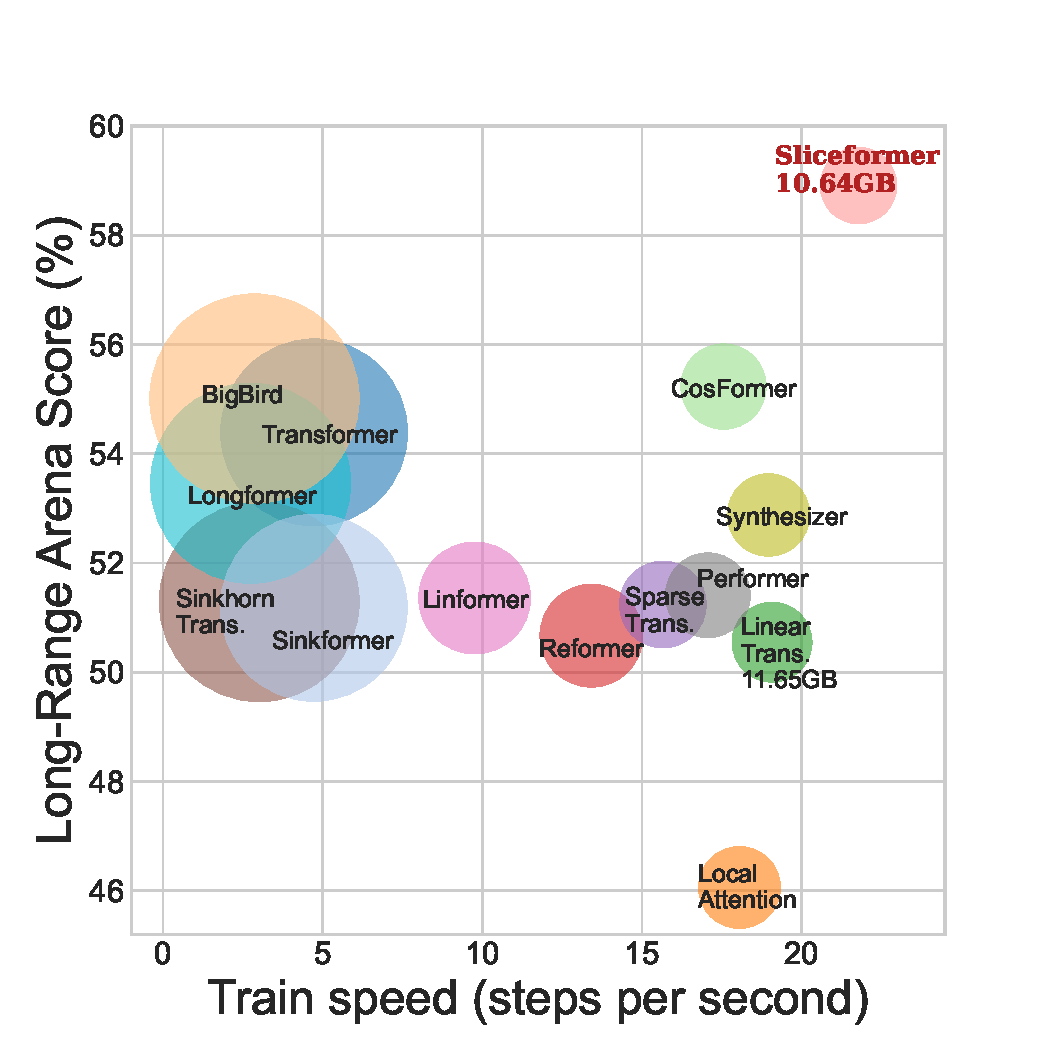
\includegraphics[width=0.46\textwidth]{figures/lra-3.pdf}
    \caption{The comparison for various Transformers and our Sliceformer on the LRA benchmark. 
    The length of sequence is 3K.
    The x-axis corresponds to the number of training steps per second. 
    The y-axis corresponds to the average score (\%) on the LRA benchmark.
    The peak memory usage of each model is represented as the area of the corresponding circle. 
    For a better comparison, the values (GB) of the top-2 models are shown.}
    \label{fig:cmp}
\end{wrapfigure}

% \begin{figure}[t]
%     \centering
%     \includegraphics{example-image-a}
%     \caption{The comparison for various Transformers and our Sliceformer. 
%     The x-axis corresponds to the number of steps per second, indicating the speed of the models. 
%     The y-axis corresponds to the average score on the LRA benchmark for each model.
%     The size of each model is represented by the size of the corresponding circle.}
%     \label{fig:cmp}
% \end{figure}

As shown in Table~\ref{tab:cmp}, our slicing-sorting operation only preserves the linear map from the input $\bm{X}$ to the value matrix $\bm{V}$. 
In addition, because of the simplicity of sorting, we do not need to design the ``multi-head'' concatenation architecture --- concatenating different linear maps is equivalent to increasing the columns of $\bm{W}_V$ directly. 
Therefore, the corresponding Sliceformer has fewer parameters and lower computational complexity compared to the Transformer and its variants. 
We analyze the connections and differences between the proposed slicing-sorting operation and the MHA mechanism and discuss its rationality in-depth. 
Specifically, we find that although abandoning the MHA mechanism, the slicing-sorting operation actually replaces the attention maps with a set of permutation matrices that are friendly to the backpropagation and have the sparsity and doubly-stochastic property. 
We test our Sliceformer in the well-known Long-Range Arena (LRA) benchmark. 
As shown in Figure~\ref{fig:cmp}, compared to the Transformer and its variants, our Sliceformer achieves superior performance with less memory cost and runtime. 
Moreover, through more analytic experiments, we demonstrate the numerical stability of our Sliceformer and its potential to large-scale classification problems.  
More details can be found in the following experimental section.
